% Set up the document
\documentclass{article}

% Page size
\usepackage[
    letterpaper,]{geometry}

% Lines between paragraphs
\setlength{\parskip}{\baselineskip}
\setlength{\parindent}{0pt}

% Math
\usepackage{mathtools}
\usepackage{amssymb}
\usepackage{commath}

% Short form for mathbf
\def\*#1{\mathbf{#1}}

% Unit vectors
\newcommand{\ihat}{\boldsymbol{\hat{\imath}}}
\newcommand{\jhat}{\boldsymbol{\hat{\jmath}}}

% Links
\usepackage{hyperref}

% Page numbers at top right
\usepackage{fancyhdr}
\pagestyle{fancy}
\fancyhf{}
\fancyhead[R]{\thepage}
\renewcommand\headrulewidth{0pt}

% Graphics
\usepackage{float}
\usepackage{graphicx}
\graphicspath{ {./img/} }

\begin{document}

\textbf{MATH 462 Homework 0} \\
\textbf{Matt Wiens \#301294492} \\
\textbf{2020-01-15}

\textbf{A)} Consider a scalar function of two variables,
%
\begin{equation*}
    \psi(x, y) = y \del{1 - \frac{1}{r^2}} + \frac{B}{2} \ln(r^2)
    ,
\end{equation*}
%
where $r^2 = x^2 + y^2$ and $B$ is a positive constant. Define a vector
field $\*U(x, y) = \del{u(x, y), v(x, y)}$ where the scalar velocity
functions $u(x, y)$ and $v(x, y)$ are related to $\psi(x, y)$ by
%
\begin{equation*}
    u(x, y) = + \pd{\psi}{y}; \quad v(x, y) = - \pd{\psi}{x}.
\end{equation*}
%
Calculate these velocities and evaluate explicitly the divergence of the
velocity field. Carry out this calculation in (i) mixed Cartesian
variables $\{x, y, r\}$ where $r$ derivatives are done implicitly, and
in (ii) purely polar coordinates $\{r, \theta\}$. Explain why the end
result could have been anticipated, and that $\*U(x, y)$ can be
represented as a curl ($\nabla \times$).


Show that $\*U(x, y)$ can also be represented by a gradient, $\nabla
\phi(x, y)$, by constructing the simplest $\phi(x, y)$. Could this
result have been anticipated, or is there something special going on?
Your end result will seem to be multi-valued, but do you think this is a
serious issue?

\textbf{Solution}

In mixed Cartesian variables we have (by repeatedly applying the chain
rule)
%
\begin{align*}
    u(x, y)
        &= \dpd{\psi}{y} \\
        &=
            \del{1 - \frac{1}{r^2}}
            + y \del{\frac{2}{r^3} \dpd{r}{y}}
            + \frac{B}{2 r^2} \del{2 r} \dpd{r}{y} \\
        &=
            1 - \frac{1}{r^2}
            + \frac{2 y^2}{r^4}
            + \frac{B y}{r^2} \\
        &=
            1
            + \frac{1}{r^2} \del{B y - 1}
            + \frac{2 y^2}{r^4}
        ,
\end{align*}
%
and
%
\begin{align*}
    v(x, y)
        &= - \dpd{\psi}{x} \\
        &=
            - \frac{2 y}{r^3} \dpd{r}{x}
            - \frac{B}{2 r^2} \del{2 r} \dpd{r}{x} \\
        &=
            - \frac{2 y x}{r^4}
            - \frac{B x}{r^2}
        .
\end{align*}
%
The divergence of the vector field is then (again calculated by
repeatedly applying the chain rule)
%
\begin{align*}
     \nabla \cdot \*U
        &= \dpd{u}{x} + \dpd{v}{y} \\
        &=
            \del{\frac{2 x}{r^4} (1 - B y) - \frac{8 x y^2}{r^6}}
            +
            \del{
                - \frac{2 x}{r^4}
                + \frac{8 x y^2}{r^6}
                + \frac{2 B x y}{r^4}
            } \\
        &= 0
        .
\end{align*}
%
Performing the same calculations in polar coordinates, we
first express $\psi$ in terms of $r$ and $\theta$:
%
\begin{equation*}
    \psi(r, \theta) = r \sin \theta \del{1 - \frac{1}{r^2}} + \frac{B}{2} \ln(r^2)
    .
\end{equation*}
%
Then we have
%
\begin{align*}
    \dpd{\psi}{r} &=
        \sin \theta
        + \frac{\sin \theta}{r^2}
        + \frac{B}{r}
        , \\
    \dpd{\psi}{\theta} &=
        r \cos \theta \del{1 - \frac{1}{r^2}}
        .
\end{align*}
%
Expressing
%
\begin{equation*}
    \*U(r, \theta) = \del{\frac{1}{r} \dpd{\psi}{\theta}, - \dpd{\psi}{r}}
    ,
\end{equation*}
%
we have
%
\begin{align*}
    r \del{\nabla \cdot \*U}
        &= \dpd{\del{r U_1}}{r} + \dpd{U_2}{\theta} \\
        &= \dpd{}{r} \del{\dpd{\psi}{\theta}} +  \dpd{}{\theta} \del{- \dpd{\psi}{r}} \\
        &= \sbr{\cos \theta \del{1 - \frac{1}{r^2}} + 2 \frac{\cos \theta}{r^2}}
           + \sbr{-\cos \theta - \frac{\cos \theta}{r^2}} \\
        &= 0
        .
\end{align*}
%
This could have been easily anticipated because mixed partial
derivatives commute. Taking Cartesian coordinates as an example, it is
obvious that
%
\begin{equation*}
    \nabla \cdot \*U = \dpd{u}{x} + \dpd{v}{y}
                     = \dpd{}{x} \dpd{\psi}{y} + \dpd{}{y} \del{- \dpd{\psi}{x}}
                     = \dmd{\psi}{2}{x}{}{y}{} - \dmd{\psi}{2}{y}{}{x}{}
                     = 0
    .
\end{equation*}
%
Note also that we can express $\*U(x, y)$ as
%
\begin{equation*}
    \*U(x, y) = \dpd{\psi}{y} \ihat - \dpd{\psi}{x} \jhat = \nabla \times \nabla \psi
    .
\end{equation*}
%
If for some function $\phi$ we have $\nabla \phi = \*U$ then we must
have
%
\begin{align*}
    \dpd{\phi}{x} &= \dpd{\psi}{y}, \\
    \dpd{\phi}{y} &= - \dpd{\psi}{x}.
\end{align*}
%
This implies that
%
\begin{align*}
    \phi(x, y) &= \int \dpd{\psi}{y} \dif x + c_1(y), \\
    \text{and } \quad \phi(x, y) &= - \int \dpd{\psi}{x} \dif y + c_2(x).
\end{align*}
%
Computing the integrals (with the help of Maple) we have
%
\begin{align*}
    \int \dpd{\psi}{y} \dif x
        &= \int
            \del{
            1
            + \frac{1}{r^2} \del{B y - 1}
            + \frac{2 y^2}{r^4}
            }
           \dif x \\
        &= x + B \arctan \del{\frac{x}{y}} + \frac{x}{r^2}, \\ \\
    - \int \dpd{\psi}{x} \dif y
        &= - \int
            \del{
            \frac{2 y x}{r^4}
            + \frac{B x}{r^2}
            }
           \dif x \\
        &=  - B \arctan \del{\frac{y}{x}} + \frac{x}{r^2} \\
        &=  - \frac{\pi B}{2} + B \arctan \del{\frac{x}{y}} + \frac{x}{r^2}
        .
\end{align*}
%
So we can take $\phi$ to be given by
%
\begin{equation*}
    \phi(x, y) = x \del{1 + \frac{1}{r^2}} + B \arctan \del{\frac{x}{y}} - \frac{\pi B}{2}
    .
\end{equation*}
%
Since we only care about taking the gradient of $\phi$, we can drop the
constant and have a simpler expression
%
\begin{equation*}
    \phi(x, y) = x \del{1 + \frac{1}{r^2}} + B \arctan \del{\frac{x}{y}}
    .
\end{equation*}
%
I emphasize again, the constant does not matter in this context! That we
can find such a $\phi$ could have been anticipated be noticing that
$\*U$ is simply a rotation (a 90-degree clockwise rotation) of $\nabla
\phi$. Thus we can view $\*U$ as representing $\phi$ in a new coordinate
system with the axes rotated relative to the original coordinate system.

\newpage

\textbf{B)} The posted Matlab script \textit{hw01.m} gives an example of
plotting level curves and vector fields. Modify the script to use the
$\psi(x, y)$ and $\*U(x, y)$ from problem A. The plot also
shows how to remove the points inside the unit circle---how does this
circle visually relate to the vector field? Note also that the plots
look qualitatively different over ranges of the parameter $B$.

Make two plots for values of $B$ that show two differing flow patterns.
Indicate by a (computed) red $\ast$ places where the velocity field is
$\*0$. Choose separate gridpoint sets for the level curves and the
vector fields to get visually useful and well-resolved plots.

\textbf{Solution}

Visually speaking, the unit circle plays an interesting role for these
plots. In the upper half plane, the speeds of the velocity field $\*U$
are relatively large and move around the circle in a clockwise circular
pattern. In the lower half plane, closer to the circle, the velocity
still proceeds from left to right ; however, for lower values of $y$ the
speeds diminish. In terms of the level curves of $\psi$, the velocity
field $\*U$ seems to follow each level curve, meaning that if a point is
on a level curve, it will stay on that curve (or at least this is how it
visually appears). The level curves seem to be related to the curvature
of the unit circle as well (exactly what this relationship is I don't
know how to express).

An interesting phenomenon happens close to $B_{\text{crit}} = 2$. When
we have values of $B < B_{\text{crit}}$, level curves intersect the unit
circle, however, for values $B > B_{\text{crit}}$, this never occurs.
Another interesting thing happens around $B_{\text{crit}} = 2$: when $B$
is less than this value the zero-velocity points always occur at $y =
- \frac{B}{2}$ \textit{on} the unit circle, and when $B$ is greater than
this value, the zero-velocity points always occur at $x = 0$
with one point above the unit circle and one point below the unit circle.

One last observation is that regardless of $B$, the level set for $\psi
= 0$ includes the unit circle itself. (This can be easily verified by
substituting $r = 1$ into the equation for $\psi$.)

Two plots are shown in
Figures~\ref{figure:b-low}~and~\ref{figure:b-high}, which show the level
curves of $\psi$ along with the velocity field $\*U$ with $B = 1.5$ and
$B = 2.5$, respectively. The size of the quivers show the magnitude of
$\*U$. The red $\ast$ points $(x, y)$ show where $\*U(x, y) = \*0$. The
contour lines plotted in black show where $\psi = 0$. Note that $\psi = 0$
always on the unit circle! This is hard to see in the plot because we
have also explicitly plotted the unit circle.
%
\begin{figure}
    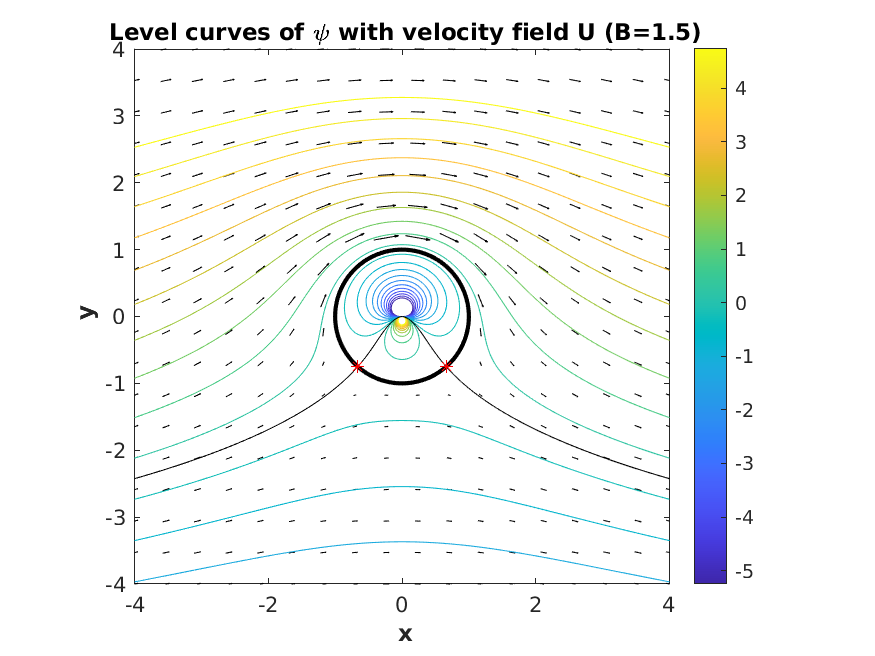
\includegraphics[width=\textwidth]{fig1}
    \centering
    \caption{Level curves of $\psi$ with velocity field $\*U$ ($B = 1.5$)}
    \label{figure:b-low}
\end{figure}
%
\begin{figure}
    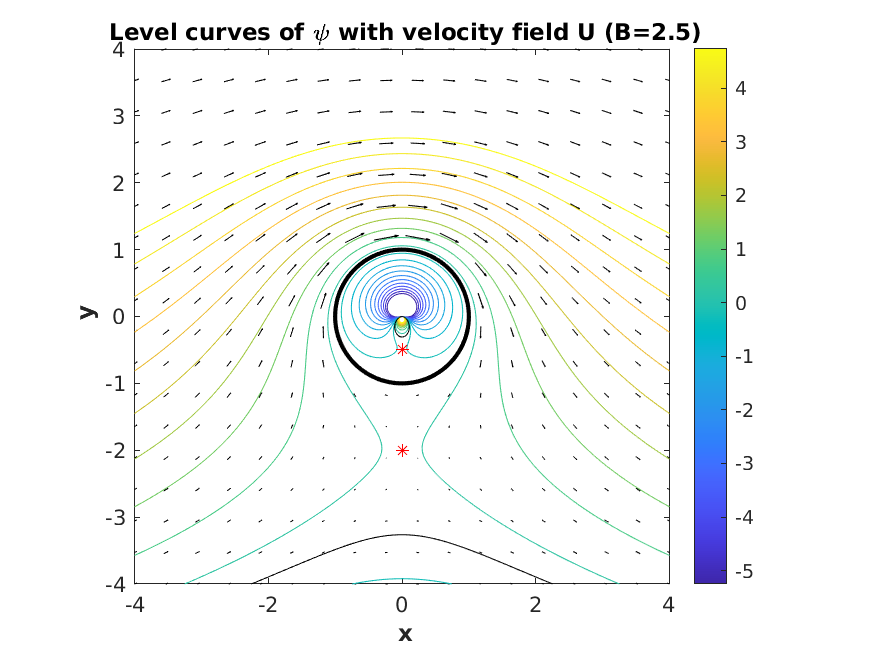
\includegraphics[width=\textwidth]{fig2}
    \centering
    \caption{Level curves of $\psi$ with velocity field $\*U$ ($B = 2.5$)}
    \label{figure:b-high}
\end{figure}

\end{document}
